\documentclass[10pt,letterpaper]{article}
\usepackage[margin=1in]{geometry}
\usepackage[T1]{fontenc}
\usepackage{lmodern,microtype,amsmath,amssymb,amsthm,booktabs,graphicx}
\usepackage[numbers,sort&compress]{natbib}
\usepackage{algorithm,algpseudocode,xcolor,xurl}
\usepackage[colorlinks=true,linkcolor=blue!45!black,citecolor=blue!45!black,urlcolor=blue!45!black]{hyperref}
\newtheorem{theorem}{Theorem}[section]
\newtheorem{lemma}[theorem]{Lemma}
\newtheorem{proposition}[theorem]{Proposition}
\newtheorem{corollary}[theorem]{Corollary}
\newcommand{\R}{\mathbb{R}}
\newcommand{\Z}{\mathbb{Z}}
\newcommand{\lat}{\mathcal{L}}
\newcommand{\pat}{\mathcal{P}}
\newcommand{\one}{\mathbf{1}}
\newcommand{\opt}{\operatorname{OPT}}
\newcommand{\LATCH}{\textsc{Latch}}
\title{Matrix-Free Lattice Fusion of\protect\\Learned Dual Certificates}
\author{Shivam Gupta\\Independent Researcher\\\texttt{shivam1720406@gmail.com}}
\date{17 October 2026}
\begin{document}
\maketitle
\begin{abstract}
A portfolio of learned dual predictions is usually reduced to its strongest feasible member. Can complementary predictions yield a stronger certificate without another pass over the optimization instance? We study exact aggregation over the coordinatewise minimum--maximum lattice generated by feasible hints. For $K$ vectors in $\R^d$, we construct a threshold-pattern poset with at most $\min\{d(K-1),2^K-2\}$ elements. Maximizing any separable objective over the generated lattice reduces to one maximum-weight closure problem on this poset, with no access to the original constraints. Applied to bipartite assignment after reversing the sign of column duals, fusion preserves feasibility and weakly improves the best input lower bound on every instance. A two-hint example separates fusion from every convex combination. We also give a two-objective hardness boundary and an explicit counterexample to runtime monotonicity. Independent enumeration verifies 4,496 small fusion cases. On 4,320 held-out synthetic assignments with learned prototype portfolios, eight-hint fusion strictly improves 4,037 certificates and ties on 283; family-level mean dual-gap reductions range from 5.81\% to 20.02\%. However, the measured reference pipeline is 2.10 times slower at the median after fusion overhead. The result is an exact certificate-aggregation primitive, with a reproducible evaluation of both its gains and its present computational limits.
\end{abstract}

\section{Introduction}
Learning-augmented optimization uses predictions to initialize exact algorithms rather than replace their correctness guarantees. For minimum-cost bipartite matching, predicted dual variables can be repaired to feasibility and passed to a primal--dual solver \citep{dinitz21}. With several predictors, a natural procedure repairs each candidate and selects the feasible dual with greatest objective value \citep{portfolios}. That procedure identifies a strong whole-vector hint. It does not combine useful coordinates of different hints.

Arbitrary coordinate selection can destroy feasibility: individually valid row and column prices may jointly exceed an edge cost. Convex averaging preserves feasibility but cannot exceed the strongest input linear objective. This leaves a precise question: \emph{can one optimize a richer, provably feasible family of combinations using only the feasible vectors themselves?} An answer should state the admissible family exactly, produce a checkable expression for the result, and account for aggregation cost separately from certificate strength.

We answer this question for feasible regions closed under coordinatewise minimum and maximum. Assignment duals have this property after reversing the column variables' signs. The generated lattice can contain many vectors, but its optimization need not enumerate them. Each coordinate changes only when a common monotone Boolean rule accepts a particular subset of predictors. Identical subsets across coordinates must receive the same decision; subset inclusion imposes an implication. Aggregating objective increments at these observed subsets yields a maximum-weight closure problem.

We call the construction \LATCH{}: lattice aggregation of certified hints. Its contribution is an explicit threshold-pattern formulation for constraint-independent fusion, its assignment-certificate interpretation, and an executable examination of where certificate improvements do and do not translate into computation savings. The lattice normal forms and maximum-closure reduction are classical \citep{birkhoff,couceiro,picard}; we do not claim those foundations, dual warm starts, or prediction portfolios as new. We prove the construction directly and compare it with the established best-feasible-member rule.

The findings support a bounded conclusion. Fusion can improve the dual certificate beyond every individual hint and every convex average, while retaining exact feasibility. It does not necessarily improve distance to a particular optimal dual, the solver's actual search trajectory, or elapsed time. Our experiments retain these distinctions: lower bounds improve consistently, yet implementation overhead exceeds the average reduction in solver work.

\begin{figure}[t]
\centering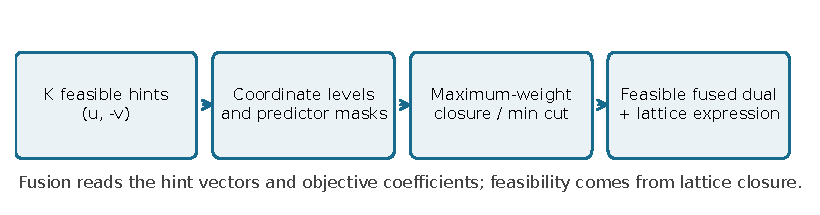
\includegraphics[width=\linewidth]{figures/workflow.pdf}
\caption{The fusion interface. Hints must already be feasible for the same instance and expressed in common coordinates. Fusion receives neither the constraint system nor the assignment cost matrix. A generated minimum--maximum expression provides a feasibility witness.}
\label{fig:workflow}
\end{figure}

\section{Related Work and Positioning}
\paragraph{Learned duals and portfolios.}
Dinitz et al.\ establish prediction-dependent exact matching algorithms and learnability results \citep{dinitz21}. Their portfolio extension repairs every hint and selects the greatest feasible dual objective \citep{portfolios}. That selection rule is our main baseline. We replace its finite candidate set with the lattice generated by those candidates. Our result concerns the additional fusion stage, conditional on already feasible hints; it does not reduce the cost of producing or repairing the portfolio. General methods for learning algorithmic predictions are developed by Khodak et al.\ \citep{khodak}.

Sakaue and Oki obtain improved prediction-dependent bounds through discrete convex analysis \citep{sakaue22}, then analyze distance to the entire optimal solution set rather than one selected optimum \citep{sakaue23}. Those results address prediction quality and warm-start complexity. We optimize a different observable quantity: the dual objective over a declared generated family. A greater dual objective alone does not imply a smaller distance to the optimal set or faster execution of every solver. Neural dual prediction and one-sided feasible completion are central to the recent RowDualNet framework \citep{rowdual}; we use simple learned prototypes to isolate fusion, without claiming a competitive neural predictor or reproducing that system's speedups.

\paragraph{Lattices and closure.}
Finite distributive lattices admit order-ideal representations \citep{birkhoff}. Lattice term functions have minimum--maximum normal forms and associated monotone Boolean rules \citep{couceiro}. Picard's closure construction converts additive weights and implications to a minimum cut \citep{picard}. Our formulation specializes these ideas to subsets actually observed at numerical coordinate thresholds. It avoids constructing the full generated lattice or all $2^K$ subsets.

\paragraph{Proposal fusion.}
Combining suboptimal solutions with graph cuts is established in fusion moves for Markov random fields \citep{lempitsky}, and fusion moves have also been combined with dual methods for quadratic graph matching \citep{graphfusion}. Our search family is a common lattice term applied to feasible dual coordinates, rather than arbitrary per-variable selection between primal proposals. The threshold-pattern formulation optimizes that family without an instance-energy or constraint oracle. We do not claim that graph-cut-based proposal fusion itself is new.

A separate, cost-aware alternative chooses each coordinate from its finite input menu while enforcing the original difference constraints. Such problems fit monotone two-variable optimization and closure methods \citep{hochbaum}. That feasible menu family can strictly contain our lattice family. It reads and encodes the original constraints; \LATCH{} instead uses only the vectors and their lattice structure. The difference is an information-access restriction, not a claim that stronger cost-aware optimization is impossible.

\section{Fusion over a Generated Numerical Lattice}
Let $z^1,\ldots,z^K\in\R^d$, with $K\geq1$. Write $x\vee y$ and $x\wedge y$ for coordinatewise maximum and minimum. Define $\lat(Z)$ as the smallest set containing $z^1,\ldots,z^K$ and closed under these two operations. Every coordinate of every resulting vector is an input value at that coordinate, so the set is finite. The same lattice expression is applied at every coordinate; coordinates cannot choose unrelated expressions.

We first maximize $a^\top x$ for arbitrary $a\in\R^d$. List coordinate $q$'s distinct input values as $t_{q,0}<\cdots<t_{q,r_q}$, with $r_q\leq K-1$. For $\ell=1,\ldots,r_q$, define
\begin{equation}
 S_{q,\ell}=\{h\in[K]:z^h_q\geq t_{q,\ell}\},\qquad
 \Delta_{q,\ell}=t_{q,\ell}-t_{q,\ell-1}.
 \label{eq:patterns}
\end{equation}
These subsets are nonempty and proper. Let $\pat$ be the distinct observed subsets, ordered by inclusion, and let $N=|\pat|$. Introduce one binary decision $b_S$ per observed subset and impose
\begin{equation}
 b_S\leq b_T\quad\text{whenever }S\subseteq T.
 \label{eq:implications}
\end{equation}
A satisfying assignment is an upward-closed selection of patterns.

\begin{lemma}[Exact threshold representation]
The vectors in $\lat(Z)$ are exactly
\begin{equation}
 x_q=t_{q,0}+\sum_{\ell=1}^{r_q}\Delta_{q,\ell}b_{S_{q,\ell}},
 \label{eq:decode}
\end{equation}
for binary assignments satisfying \eqref{eq:implications}.
\label{lem:representation}
\end{lemma}
\begin{proof}
For a lattice expression $F$, thresholding commutes with minimum and maximum: minimum becomes Boolean AND and maximum becomes Boolean OR. Thus $[F(z^1_q,\ldots,z^K_q)\geq t]$ equals a common monotone Boolean term evaluated at $\{h:z^h_q\geq t\}$. Its restriction to $\pat$ satisfies \eqref{eq:implications}. Summing accepted level increments gives \eqref{eq:decode}.

Conversely, let $Q=\{S\in\pat:b_S=1\}$ be upward closed within $\pat$. Define
\begin{equation}
 F_Q(z^1,\ldots,z^K)
 =\bigvee_{S\in Q\cup\{[K]\}}\ \bigwedge_{h\in S}z^h.
 \label{eq:dnf}
\end{equation}
The $[K]$ term makes this expression well defined even for empty $Q$. At an observed proper subset $T$, its Boolean threshold value is one exactly when some selected $S\subseteq T$. A selected $T$ witnesses itself; conversely, upward closure forces any such $T$ to be selected. The $[K]$ term cannot activate at a proper $T$. Threshold decisions therefore agree exactly with $b_T$, proving \eqref{eq:decode} and membership in $\lat(Z)$.
\end{proof}

\begin{theorem}[Pattern-cut fusion]
For rational vectors and rational coefficients, maximizing $a^\top x$ over $\lat(Z)$ reduces to one minimum $s$--$t$ cut on a graph with $N+2$ vertices and at most $N(N-1)+2N$ arcs, where
\begin{equation}
 N\leq\min\{d(K-1),2^K-2\}.
 \label{eq:size}
\end{equation}
Construction and decoding require no description of the original feasible region. The result includes an expression of the form \eqref{eq:dnf}.
\label{thm:cut}
\end{theorem}
\begin{proof}
Substitute \eqref{eq:decode} into the objective:
\begin{equation}
 a^\top x=B+\sum_{S\in\pat}w_Sb_S,\quad
 B=\sum_q a_qt_{q,0},\quad
 w_S=\sum_{(q,\ell):S_{q,\ell}=S}a_q\Delta_{q,\ell}.
 \label{eq:weights}
\end{equation}
Create an arc $S\to T$ for every strict inclusion among observed patterns. An allowable selection is exactly a closure. Connect the source to each positive-weight node with capacity $w_S$, and each negative-weight node to the sink with capacity $-w_S$. Give implication arcs capacity $H=1+\sum_S|w_S|$. A cut crossing no implication arc exists and costs at most $\sum_S|w_S|$, so no minimum cut crosses an implication arc. Its source-side pattern set is upward closed and maximizes total weight. If the cut capacity is $c_{\min}$, the optimal value is
\begin{equation}
 B+\sum_{S:w_S>0}w_S-c_{\min}.
 \label{eq:certificate}
\end{equation}
Lemma~\ref{lem:representation} supplies the vector and expression. Each coordinate contributes at most $K-1$ patterns, and only $2^K-2$ nonempty proper subsets exist. Rational capacities may be scaled to integers without changing the optimal selections.
\end{proof}

Sorting costs $O(dK\log K)$ comparisons. A sweep forms masks and increments; constructing inclusion arcs uses $O(N^2)$ subset tests. These count arithmetic and subset operations; arbitrary-length masks and rational capacities have their usual bit costs. The graph is polynomial in input dimensions because $N\leq d(K-1)$. For fixed $K$, its vertex count is also independent of $d$; for eight hints it is at most 254. The generated lattice itself can have many more than $N$ elements.

\begin{algorithm}[t]
\caption{\LATCH{} for a linear objective}
\begin{algorithmic}[1]
\Require Vectors $Z=(z^1,\ldots,z^K)$ and coefficients $a$
\State Sort distinct coordinate levels; form observed masks $S_{q,\ell}$
\State Accumulate $B,w_S$ and create arcs $S\to T$ for observed $S\subset T$
\State Add signed weight arcs and compute a minimum $s$--$t$ cut
\State Let $Q$ be its source-side pattern set
\State Decode $x$ by \eqref{eq:decode}; retain $Q$ as an expression witness
\State \Return $x$, $a^\top x$, $Q$, and the cut value
\end{algorithmic}
\end{algorithm}

\begin{corollary}[Feasibility and dominance]
If all input vectors belong to a common set $P$ closed under $\vee,\wedge$, the fused vector belongs to $P$ and satisfies
\[
 a^\top x_{\LATCH}\geq\max_h a^\top z^h
 =\max_{x\in\operatorname{conv}(Z)}a^\top x.
\]
Adding a hint cannot decrease the optimum; duplicating or reordering hints leaves its value unchanged.
\label{cor:dominance}
\end{corollary}
\begin{proof}
Closure gives $\lat(Z)\subseteq P$, and every input belongs to $\lat(Z)$. A linear objective's convex-hull maximum is an input maximum. Adding a generator enlarges the lattice; duplication and reordering do not change it.
\end{proof}

\begin{proposition}[Separable scores and stability]
The same graph optimizes $\sum_q g_q(x_q)$ for arbitrary real-valued functions specified on coordinate menus, using
\[
 w_S=\sum_{(q,\ell):S_{q,\ell}=S}
 [g_q(t_{q,\ell})-g_q(t_{q,\ell-1})].
\]
For a linear objective, if $\max_{h,q}|z^h_q-\widetilde z^h_q|\leq\epsilon$, the optimal fusion values differ by at most $\|a\|_1\epsilon$.
\end{proposition}
\begin{proof}
Accepted levels in a coordinate form an initial segment: predictor subsets decrease with increasing thresholds, and the Boolean rule is monotone. Function-value increments therefore telescope to $g_q(x_q)$. For stability, every minimum--maximum expression is nonexpansive in the maximum norm of its inputs. Evaluating a first-array optimal expression on the second changes its linear value by at most $\|a\|_1\epsilon$. Reverse the roles for the opposite inequality. The selected expression and vector need not vary continuously.
\end{proof}

\section{Application to Exact Assignment}
For square integer $C\in\Z^{n\times n}$, the assignment dual is
\begin{equation}
 \max_{u,v}\ \sum_i u_i+\sum_jv_j
 \quad\text{subject to}\quad u_i+v_j\leq C_{ij}.
 \label{eq:assignment}
\end{equation}
Set $z=(u,-v)$ and $a=(\one_n,-\one_n)$. The constraints become $z_i-z_{n+j}\leq C_{ij}$ and the objective is $a^\top z$.

\begin{lemma}[Difference-constraint closure]
The set $\{x:x_p-x_q\leq c\}$ is closed under coordinatewise minimum and maximum. Hence transformed feasible assignment duals form a sublattice.
\end{lemma}
\begin{proof}
If $x_p\leq x_q+c$ and $y_p\leq y_q+c$, then $\max(x_p,y_p)\leq\max(x_q,y_q)+c$ and $\min(x_p,y_p)\leq\min(x_q,y_q)+c$. Intersections preserve closure.
\end{proof}

The sign reversal is essential: maximizing both \emph{original} row and column duals is generally invalid. A transformed join takes maximum row duals and minimum column duals. The fused result is a rigorous lower bound on the optimal assignment cost.

\paragraph{Strict separation from convex averages.}
For $C=\left(\begin{smallmatrix}1&2\\2&1\end{smallmatrix}\right)$, consider feasible transformed hints
\[
 z^1=(1,-2,0,-1),\qquad z^2=(-2,1,-1,0).
\]
Both have objective zero, as does every convex combination. Their join is $(1,1,0,0)$, with objective two, equal to the diagonal assignment cost. Scaling all costs and hints by a positive integer makes the additive improvement arbitrarily large. This separates certified bounds, not runtime lower bounds for competing solvers.

\paragraph{Primal--dual improvement phases.}
Let $D^*=\opt(C)$ and $D(z)=a^\top z$. In the integer primal--dual analysis for learned matching \citep{dinitz21,portfolios}, each positive phase increases the dual objective by at least one. Its number of improvement phases is at most $D^*-D(z)$. Fusion weakly improves this \emph{upper bound} relative to the best portfolio member. It does not order actual phase counts, zero-increment loops, or wall time. Appropriate accounting is
\[
 T_{\rm total}=T_{\rm repair}+T_{\rm fusion}+T_{\rm exact\ solver}.
\]
The fusion theorem gives neither a new sample-complexity bound nor a guarantee that this total beats a cold-start solver.

\paragraph{The coordinate-menu limitation.}
For $C=\one_{2\times2}$, let $z^1=(1,0,0,1)$ and $z^2=(0,1,1,0)$. Both are feasible and their generated lattice has objective zero throughout. The feasible coordinate-menu splice $(1,1,0,0)$ has value two but lies outside that lattice: coordinates one and four agree in both inputs and remain equal in every common lattice expression. Optimizing all feasible menu splices is therefore a distinct, cost-aware problem. One-sided completion of fused row variables can also strengthen a bound by reading $C$ again.

\section{A Boundary: Two Coupled Scores}
The additive pattern-weight construction does not automatically extend to a conservative choice between coupled score scenarios.
\begin{theorem}[Two-score hardness]
For binary input vectors and two integer coefficient vectors $a,b$, maximizing $\min\{a^\top x,b^\top x\}$ over $x\in\lat(Z)$ is NP-hard, even with $K=O(\log d)$ input vectors.
\end{theorem}
\begin{proof}
Reduce from \textsc{Partition} \citep{karp}. For positive integers $w_1,\ldots,w_m$ with even total $W$, choose $K$ with $\binom{K}{\lfloor K/2\rfloor}\geq m$. Choose distinct subsets $S_1,\ldots,S_m\subset[K]$ of size $\lfloor K/2\rfloor$, and define $K$ binary vectors in dimension $m+1$ by $z^h_i=[h\in S_i]$ for $i\leq m$ and $z^h_{m+1}=1$. The observed threshold patterns form an antichain. Lemma~\ref{lem:representation} implies that every vector in $\{0,1\}^m\times\{1\}$ is attainable. Define
\[
 A(x)=\sum_{i=1}^m w_ix_i,\qquad
 B(x)=Wx_{m+1}-\sum_{i=1}^m w_ix_i.
\]
Their minimum reaches $W/2$ exactly for an equal partition. Taking $K=2\lceil\log_2(2m)\rceil$ supplies enough middle-level subsets with polynomial construction size and $K=O(\log m)$. Odd-total instances map to a fixed no-instance. This proves the stated hardness, without asserting strong NP-hardness or hardness for fixed constant $K$.
\end{proof}
This boundary concerns general fusion with a nonseparable objective, not the single assignment-dual objective.

\section{Experimental Design}
We examine correctness, certificate strength, and overhead separately. All main assignment experiments use integer arithmetic. Generators, frozen prototype banks, cost hashes, outputs, and figure scripts accompany the paper.

\paragraph{Independent checks.}
An enumerator begins with input tuples and repeatedly inserts pairwise coordinate minima and maxima until closure. It uses neither patterns nor flow. Its exact optimum is compared with fusion on all 512 binary $3\times3$ arrays under all eight sign objectives (4,096 cases) and on 400 seeded integer arrays with $K\in\{1,2,3,4\}$ and dimension six. A separate reconstruction evaluates the returned minimum--maximum expression coordinate by coordinate. On 500 random assignment instances, with negative as well as positive costs and $n\in\{2,3,4,8,16\}$, six solver starts must agree with SciPy's independent exact assignment routine \citep{scipy}. Additional tests cover duplicate and reordered hints, nested portfolios, stability, the antichain reduction, the menu limitation, and runtime nonmonotonicity.

\paragraph{Learning and completion.}
For each of three seeds, three sizes $n\in\{16,32,64\}$, and three families, we generate 240 training assignments. The reference Hungarian solver supplies optimal row duals. We subtract their integer-truncated row median to fix a gauge, cluster into eight groups using $K$-means (ten initializations, fixed random state), and retain the rounded coordinate median within each cluster. This is a simple prototype-learning baseline, not exact optimization of a portfolio-learning objective. Training solves 6,480 assignments. All predictors are frozen before evaluation.

For a test matrix, a predicted row vector $\widehat u$ is made feasible by standard one-sided completion,
\begin{equation}
 \widehat v_j=\min_i(C_{ij}-\widehat u_i).
 \label{eq:repair}
\end{equation}
All eight completions precede selection or fusion. Optimal test assignments are used only for evaluation, never for learning, completion, selection, or fusion. Identities persist across training and test; the experiments do not establish transfer to unseen sizes or identity permutations.

\paragraph{Generated distributions.}
\emph{Block} matrices have four persistent groups, cost 20 within groups and 70 across groups, independent Gaussian row-group and column-group shifts of standard deviation 12, and exponential edge noise of mean 14. Under shift, row-group deviation becomes 30 and edge-noise mean becomes 35. \emph{Spatial} matrices use supply points on the unit circle and demand points perturbed from corresponding circle sites. Cost is 100 times Euclidean distance plus uniform edge noise in $[0,20]$. Demand-coordinate noise deviation is 0.3 in the matched regime and 0.8 under shift. \emph{IID} costs are exponential draws of mean 100, increased to 250 under shift. Costs are rounded to nearest integers. These are generated assignments, not observed operational workloads.

Each of 27 learned banks is tested on 80 fresh matched and 80 shifted matrices, totaling 4,320 held-out assignments. A small exploratory pilot preceded this fixed run; the study is not preregistered. Test randomness continues each configuration's seeded generator after training. Reproduction commands and cost hashes specify this convention.

\paragraph{Policies and measurements.}
Eleven policies are retained: a row-minimum cold start; best-of-eight feasible hints; a safely rounded convex mean; a safely rounded coordinate median; join and meet of eight; one-sided completion of mean row duals; fusion of the first two, four, and eight prototypes; and completion of eight-hint fused row duals. Smaller fusion banks are nested prefixes of the frozen eight-prototype bank. The primary comparison is \LATCH{}-8 against best-of-eight. Further completion is a cost-aware certificate ablation.

All starts use the same readable dense shortest-augmenting-path Hungarian solver. We retain inner-loop counts, positive updates, exact results, and elapsed time. SciPy's compiled modified Jonker--Volgenant routine supplies the reference optimum. Best-of-eight pipeline time includes eight completions and solving; fusion adds its measured aggregation time. Tiny scoring and dictionary-bookkeeping operations lie outside those timed sections. Completion ablations are excluded from pipeline-speed claims because their extra completion time is not separately recorded. Offline training is excluded from online timing without assuming free training in deployment.

The environment is Python 3.9.6, NumPy 1.26.4, SciPy 1.13.1, and scikit-learn 1.5.0 on ARM64 macOS. Main timings are single measurements in a fixed policy order and are descriptive, not a controlled performance benchmark. We report bank seed ranges rather than treating cases sharing a learned bank as independent training replicates. A separate fusion-only scaling run takes eleven measurements after warm-up, for $K\in\{2,4,8\}$ and $d\in\{128,512,2048,8192,32768\}$.

\section{Results}
\paragraph{Correctness.}
All 4,496 fusion comparisons agree with independent enumeration. All 3,000 starts in the separate assignment suite and all 47,520 main starts attain the exact SciPy objective. Final duals are feasible and equal their matching costs. These finite checks corroborate the implementation and do not replace proofs.

\begin{table}[t]
\centering\small
\caption{Eight-hint fusion versus best-of-eight. Each row has 720 instances across three sizes and three learned banks. Gap is $\opt(C)-D(z)$; reduction compares row means. Strict counts greater fused bounds. Time is the median paired pipeline ratio; values above one mean fusion is slower.}
\label{tab:main}
\begin{tabular}{llrrrrr}\toprule
Family & Regime & Best gap & Fused gap & Reduction (\%) & Strict & Time ratio\\\midrule
Block & Matched & 30.04 & 24.58 & 18.17 & 708/720 & 1.87\\
Block & Shift & 141.72 & 129.99 & 8.28 & 588/720 & 1.94\\
Spatial & Matched & 138.56 & 110.82 & 20.02 & 706/720 & 2.09\\
Spatial & Shift & 169.23 & 144.62 & 14.55 & 652/720 & 1.96\\
IID & Matched & 61.24 & 51.76 & 15.47 & 705/720 & 2.73\\
IID & Shift & 143.48 & 135.14 & 5.81 & 678/720 & 2.49\\
\bottomrule

\end{tabular}
\end{table}

\paragraph{Certificate strength.}
Fusion strictly improves the best lower bound on 4,037 instances (93.45\%) and ties on 283, with no decreases. Family--regime mean dual-gap reductions range from 5.81\% to 20.02\% (Table~\ref{tab:main}). Matched block, spatial, and IID reductions are 18.17\%, 20.02\%, and 15.47\%; shifted reductions are 8.28\%, 14.55\%, and 5.81\%. Figure~\ref{fig:gap} shows size dependence and bank variability. These are reductions in an initial optimization gap, not in final assignment cost: all exact runs return the same optimum.

Across separately trained banks, matched spatial reductions range from 19.65\% to 20.46\%, while shifted block reductions range from 5.60\% to 9.96\%. The theorem guarantees dominance under shift but does not ensure that the portfolio remains useful or its relative gain persists in deployment.

\begin{figure}[t]
\centering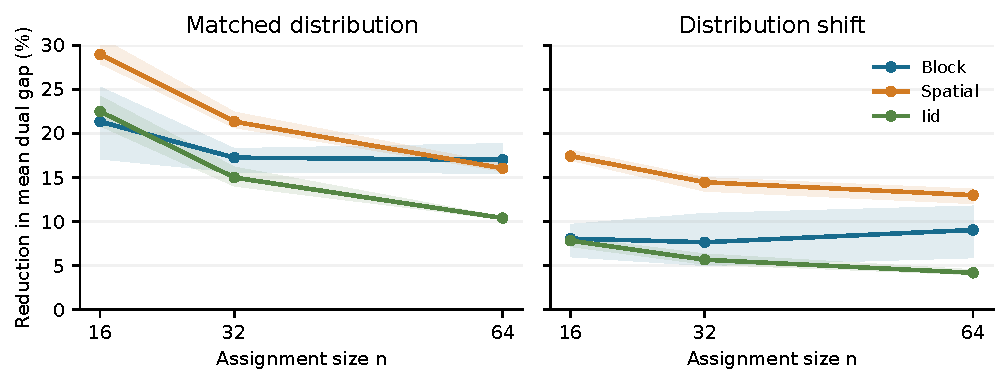
\includegraphics[width=\linewidth]{figures/gap.pdf}
\caption{Reduction in mean dual gap relative to the best feasible input. Points average the three bank-specific relative reductions at each size; shading spans their minimum and maximum. Shading is a seed range, not a confidence interval.}
\label{fig:gap}
\end{figure}

\paragraph{Search effort and time.}
Fusion uses fewer inner loops on 2,354 instances, the same number on 582, and more on 1,384. Mean loops are 115.10 versus 119.17 for the best input, a 3.42\% pooled-mean reduction. Median fusion cost is 1.381\,ms. Including common completions, fusion, and solving, the median paired time ratio is 2.10. All six group median ratios exceed one (Figure~\ref{fig:runtime}). The implementation demonstrates stronger certificates, not an end-to-end acceleration.

SciPy's compiled routine has median time 0.0294\,ms on these small matrices. It is both a correctness reference and a practical baseline: Python-level fusion and solving are not competitive here. Fixed timing order and host scheduling further limit individual-ratio interpretation.

\begin{figure}[t]
\centering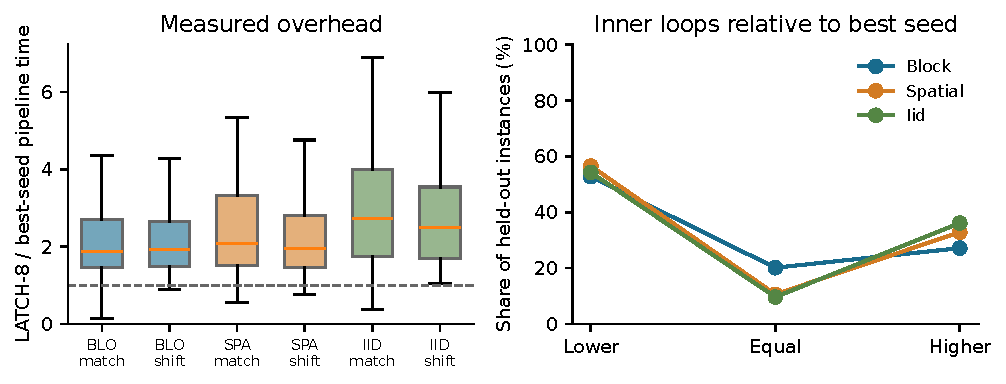
\includegraphics[width=\linewidth]{figures/runtime.pdf}
\caption{Certificate strength and runtime differ. Left: paired pipeline ratios; boxes show quartiles and medians, with 1.5-IQR whiskers and outlier markers suppressed. Right: lower, equal, or higher inner-loop counts relative to the best input, pooled across both regimes within each family.}
\label{fig:runtime}
\end{figure}

\paragraph{A nonmonotone trajectory.}
A retained four-by-four case improves the initial bound from 2 to 10 while the optimum is 12, yet increases inner loops from six to eight. Positive updates fall from four to two. Appendix~\ref{app:counterexample} gives the exact case. A better objective-gap bound cannot be reported as a universal ordering of actual search work.

\paragraph{Ablations and scaling.}
Mean gaps for best-of-eight, join, meet, safely rounded mean, and median are 114.05, 165.59, 211.37, 216.30, and 193.29, versus 99.49 for eight-hint fusion. Two- and four-hint fusion have gaps 144.00 and 120.66; their smaller banks are not expected to dominate best-of-eight. The nested-lattice guarantee applies instancewise to the two-, four-, and eight-hint fused outputs. Further cost-aware completion lowers the eight-hint mean gap to 98.13, exposing the restriction of the lattice family.

In fusion-only scaling on arbitrary integer vectors, the eight-hint graph reaches 254 pattern vertices and stays there as dimension increases (Figure~\ref{fig:scaling}). Median times rise from 8.74\,ms at dimension 128 to 75.89\,ms at 32,768. These inputs expose more patterns than the learned banks and have different timings. The fixed-$K$ graph bound does not remove vector reading, sorting, checking, or decoding cost.

\begin{figure}[t]
\centering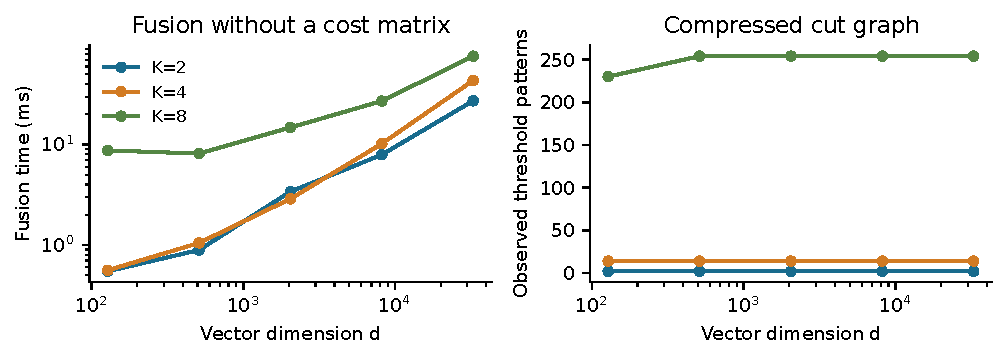
\includegraphics[width=\linewidth]{figures/scaling.pdf}
\caption{Fusion-only scaling on random integer vectors. Left: median of eleven timed runs after warm-up. Right: observed pattern vertices, excluding source and sink. No optimization cost matrix is supplied.}
\label{fig:scaling}
\end{figure}

\section{Practical Scope and Limitations}
Repeated assignment and balanced transportation in dispatch, resource allocation, and tracking offer potential applications when multiple feasible dual hints already exist. Fusion exposes complementary certificate information, supplies a lower bound for an exact optimizer, and preserves feasibility without transporting the constraint system. One possible systems use is aggregation where instance data are costly to revisit. Establishing its value requires measuring data movement, hint production, repair, aggregation, and exact completion together; our synthetic results do not establish those deployment benefits.

All hints must refer to the same instance and coordinate meanings. Input feasibility must already be established; the expression does not authenticate an incorrect upstream certificate. Closure must hold in the chosen coordinates. Rectangular assignments, capacities, and side constraints need separate analysis. A common gauge shift preserves the assignment objective and commutes with fusion expressions, but independently shifting individual hints can change their generated lattice. Our median-zero training convention fixes a gauge without optimizing it.

The lattice can omit stronger feasible coordinate-menu combinations. Value stability does not imply expression stability. Two-score hardness prevents a direct general claim for coupled robust scores. The portfolios are simple prototypes on generated families and small matrices: they establish neither a superior predictor architecture nor commercial workload performance. Current evidence supports exact aggregation and certificate-quality gains; faster implementations and broader workload evaluation remain open.

\section{Conclusion}
Complementary feasible hints can yield a certificate that best-member selection and convex averaging cannot recover. Their generated numerical lattice admits an explicit threshold-pattern minimum-cut formulation that reads only the hints and objective coefficients. For assignment duals, the result is feasible and at least as strong as the best input on every instance. Experiments confirm dual-gap reductions while exposing an unfavorable current runtime tradeoff, separating a proved aggregation benefit from an engineering benefit that remains to be demonstrated.

\paragraph{Reproducibility artifact.}
Source, retained outputs, exact checks, figure scripts, and build instructions are available at \url{https://github.com/shi1720/latch-dual-fusion}. There are no external data downloads in the experiment workflow.

\begin{thebibliography}{20}\small
\setlength{\itemsep}{3pt}
\bibitem{dinitz21} M. Dinitz, S. Im, T. Lavastida, B. Moseley, and S. Vassilvitskii. Faster Matchings via Learned Duals. \emph{Advances in Neural Information Processing Systems}, 34:10393--10406, 2021. \url{https://arxiv.org/abs/2107.09770}.
\bibitem{portfolios} M. Dinitz, S. Im, T. Lavastida, B. Moseley, and S. Vassilvitskii. Algorithms with Prediction Portfolios. \emph{Advances in Neural Information Processing Systems}, 35:20273--20286, 2022. \url{https://arxiv.org/abs/2210.12438}.
\bibitem{khodak} M. Khodak, M.-F. Balcan, A. Talwalkar, and S. Vassilvitskii. Learning Predictions for Algorithms with Predictions. \emph{Advances in Neural Information Processing Systems}, 35, 2022. \url{https://proceedings.neurips.cc/paper_files/paper/2022/hash/17061a94c3c7fda5fa24bbdd1832fa99-Abstract-Conference.html}.
\bibitem{sakaue22} S. Sakaue and T. Oki. Discrete-Convex-Analysis-Based Framework for Warm-Starting Algorithms with Predictions. \emph{Advances in Neural Information Processing Systems}, 35, 2022. \url{https://arxiv.org/abs/2205.09961}.
\bibitem{sakaue23} S. Sakaue and T. Oki. Rethinking Warm-Starts with Predictions: Learning Predictions Close to Sets of Optimal Solutions for Faster $\mathrm{L}$-/$\mathrm{L}^{\natural}$-Convex Function Minimization. \emph{Proceedings of Machine Learning Research}, 202:29760--29776, 2023. \url{https://proceedings.mlr.press/v202/sakaue23a.html}.
\bibitem{rowdual} I. Yavlovich, J. Agbaria, M. Mhamed, J. Yallouz, and N. Weinberger. Learning-Augmented Scalable Linear Assignment Problem Optimization via Neural Dual Warm-Starts. arXiv:2605.09382, 2026. \url{https://arxiv.org/abs/2605.09382}.
\bibitem{birkhoff} G. Birkhoff. Rings of Sets. \emph{Duke Mathematical Journal}, 3(3):443--454, 1937. \href{https://doi.org/10.1215/S0012-7094-37-00334-X}{doi:10.1215/S0012-7094-37-00334-X}.
\bibitem{couceiro} M. Couceiro and J.-L. Marichal. Polynomial Functions over Bounded Distributive Lattices. \emph{Journal of Multiple-Valued Logic and Soft Computing}, 18(3--4):247--256, 2012. \url{https://arxiv.org/abs/0901.4888}.
\bibitem{picard} J.-C. Picard. Maximal Closure of a Graph and Applications to Combinatorial Problems. \emph{Management Science}, 22(11):1268--1272, 1976. \href{https://doi.org/10.1287/mnsc.22.11.1268}{doi:10.1287/mnsc.22.11.1268}.
\bibitem{hochbaum} D. S. Hochbaum. Applications and Efficient Algorithms for Integer Programming Problems on Monotone Constraints. \emph{Networks}, 77(1):21--49, 2021. \href{https://doi.org/10.1002/net.21983}{doi:10.1002/net.21983}.
\bibitem{scipy} SciPy contributors. \texttt{scipy.optimize.linear\_sum\_assignment}, SciPy 1.13.1 documentation. Algorithmic reference: D. F. Crouse, On Implementing 2D Rectangular Assignment Algorithms, \emph{IEEE Transactions on Aerospace and Electronic Systems}, 52(4):1679--1696, 2016. \href{https://doi.org/10.1109/TAES.2016.140952}{doi:10.1109/TAES.2016.140952}.
\bibitem{lempitsky} V. Lempitsky, C. Rother, S. Roth, and A. Blake. Fusion Moves for Markov Random Field Optimization. \emph{IEEE Transactions on Pattern Analysis and Machine Intelligence}, 32(8):1392--1405, 2010. \href{https://doi.org/10.1109/TPAMI.2009.143}{doi:10.1109/TPAMI.2009.143}.
\bibitem{graphfusion} L. Hutschenreiter, S. Haller, L. Feineis, C. Rother, D. Kainm{\"u}ller, and B. Savchynskyy. Fusion Moves for Graph Matching. \emph{Proceedings of the IEEE/CVF International Conference on Computer Vision}, 2021. \url{https://arxiv.org/abs/2101.12085}.
\bibitem{karp} R. M. Karp. Reducibility among Combinatorial Problems. In \emph{Complexity of Computer Computations}, pp.\ 85--103, 1972. \href{https://doi.org/10.1007/978-1-4684-2001-2_9}{doi:10.1007/978-1-4684-2001-2\_9}.
\end{thebibliography}

\clearpage\appendix
\section{Exact Runtime Counterexample}\label{app:counterexample}
Consider
\[
 C=\begin{pmatrix}6&0&5&3\\8&6&3&2\\7&5&3&9\\7&4&8&8\end{pmatrix},\quad
 \begin{aligned}
 z^1&=(0,-3,5,-5,\ -2,0,2,-3),\\
 z^2&=(4,-1,-3,4,\ -2,4,-1,1),\\
 z^3&=(2,6,-5,-2,\ -2,2,3,4).
 \end{aligned}
\]
All three hints satisfy $z_i-z_{4+j}\leq C_{ij}$; their values are $0,2,-6$. Fusion returns their join
\[
 z^{\rm fused}=(4,6,5,4,\ -2,4,3,4),\qquad D(z^{\rm fused})=10.
\]
The assignment optimum is 12. With ascending row order and first-minimum column tie breaking as specified in code, the solver uses six inner loops and four positive updates from $z^2$, versus eight inner loops and two positive updates from the fused hint. This case was located by seeded search and retained as an exact regression test, not an estimate of prevalence.

\section{Implementation and Reproduction}
\paragraph{Exact scope.}
The theorem permits rational inputs. The implementation supports integers, uses Python integers for scalar certificates, and guards NumPy arithmetic and compiled max-flow capacities against overflow. Implication capacity is $1+\sum_S|w_S|$; capacities at or above $2^{30}$ are rejected rather than silently narrowed. The implementation supports at most 20 predictors. These are implementation restrictions, not theorem limits. Rational use needs an exact-capacity backend or a declared scaling and error analysis.

Zero-weight vertices are retained because deleting one without preserving induced implications can change feasible selections. Ties contribute no zero-length transitions. The all-predictor subset is not an observed threshold vertex; it occurs in reconstruction. For $K=1$, the graph has no pattern vertices and returns the input.

\paragraph{Seeds and normalization.}
For bank $s\in\{0,1,2\}$, size $n$, and family code $f\in\{1,2,3\}$ (block, spatial, IID), the generator seed is $1720406+100000s+100n+f$. It draws 240 training matrices, then 80 matched and 80 shifted tests. Clustering random state is 1720406; labels define prototype order. All policies share each test matrix. Gauge normalization subtracts the integer-truncated training row median before clustering. No test-optimal gauge is selected.

\begin{table}[H]
\centering\small
\caption{Pooled descriptive means across 4,320 assignments. Pooling raw gaps is scale dependent; within-family comparisons appear in the main table. ``Complete'' includes another cost-matrix pass.}
\begin{tabular}{lrrr}\toprule
Start & Dual gap & Inner loops & Positive updates\\\midrule
Cold row minimum &344.03&202.84&55.05\\
Best of eight &114.05&119.17&29.52\\
Safely rounded convex mean &216.30&122.19&55.50\\
Safely rounded median &193.29&123.80&45.91\\
Join of eight &165.59&130.95&33.89\\
Meet of eight &211.37&124.79&39.27\\
Mean rows, complete &152.02&128.38&32.06\\
\LATCH{}-2 &144.00&125.63&32.01\\
\LATCH{}-4 &120.66&119.49&29.82\\
\LATCH{}-8 &99.49&115.10&27.46\\
\LATCH{}-8, complete &98.13&115.28&26.96\\\bottomrule
\end{tabular}
\end{table}

\paragraph{Reproduction.}
The repository README gives exact commands, dependencies, and entry points for independent verification, retraining, evaluation, and figure generation. Retained records generate the reported figures. Re-execution should reproduce integer objectives, hints, and cost hashes in the recorded environment; elapsed times vary by host.
\end{document}
